% !TeX spellcheck = en_GB
\documentclass[11pt]{article}
\usepackage{graphicx}
\usepackage{listings}
\title{Machine Learning Project\\Task 2}
\author{Duy Nguyen Dinh \\ dinh@rhrk.uni-kl.de\and
	Minh Duc Duong\\ duong@rhrk.uni-kl.de\and
    ---\\ ---}
\date{\today}
\begin{document}

\maketitle

\section{Data Pre-processing}

\subsection{Extract vintage from "title" column}
As the task sheet requires, we need to extract the vintage from the title column. First it is necessary to identify how would vintage appears in the title. Because they indicate a specific year, they appear mostly as a concatenation of 4 digits. The process can be done by searching for numbers using regular expression ([0-9][0-9][0-9][0-9]) in each entry of title column. This is however not enough for the exaction as there can be the case, where the 4 digits do not make any sense of year (for example: 1000 or 9000 as these should not be a reasonable years for vintage). Thus, we add some constrains with the expectation of getting more meaningful numbers for the vintage. The extracted number first should be in between 1800 and 2022 because it makes more sense that all wines were made in this year range. Also there are time when we could extracted 2 or more years in the same title entry. Here we focus on the exception with 2 different numbers. The entry 2262 in the data has 2 different years (1637 and 2002). Our implementation is to extract the maximum number as vintage, which suits this entry well because 1637 represents the establish year of the facility and 2002 is the actual wine year.

It is important to keep in mind that the extraction may not absolute accurate because the idea for the extraction of vintage comes through the observation of the data frame. For the better result, data should be consistent with a recognizable pattern.

\subsection{Histogram}
Plotting is one way to get an overview of the values of each column. There will be two types of plotting depend on the value type of columns. For numeric types (Integer or Float), we plot histograms which show the range and the distribution of values. For string type, we plot the counts of each unique values.

All histogram for numeric columns are plotted with group of 3 bins. Because there can be too many unique values to plot, we decided to plot the counts of top 20 unique values for string columns. We also exclude description and title columns from the plot result with the assumption that each entry of these columns are unique and this makes plotting for these columns serves no purpose.

Country

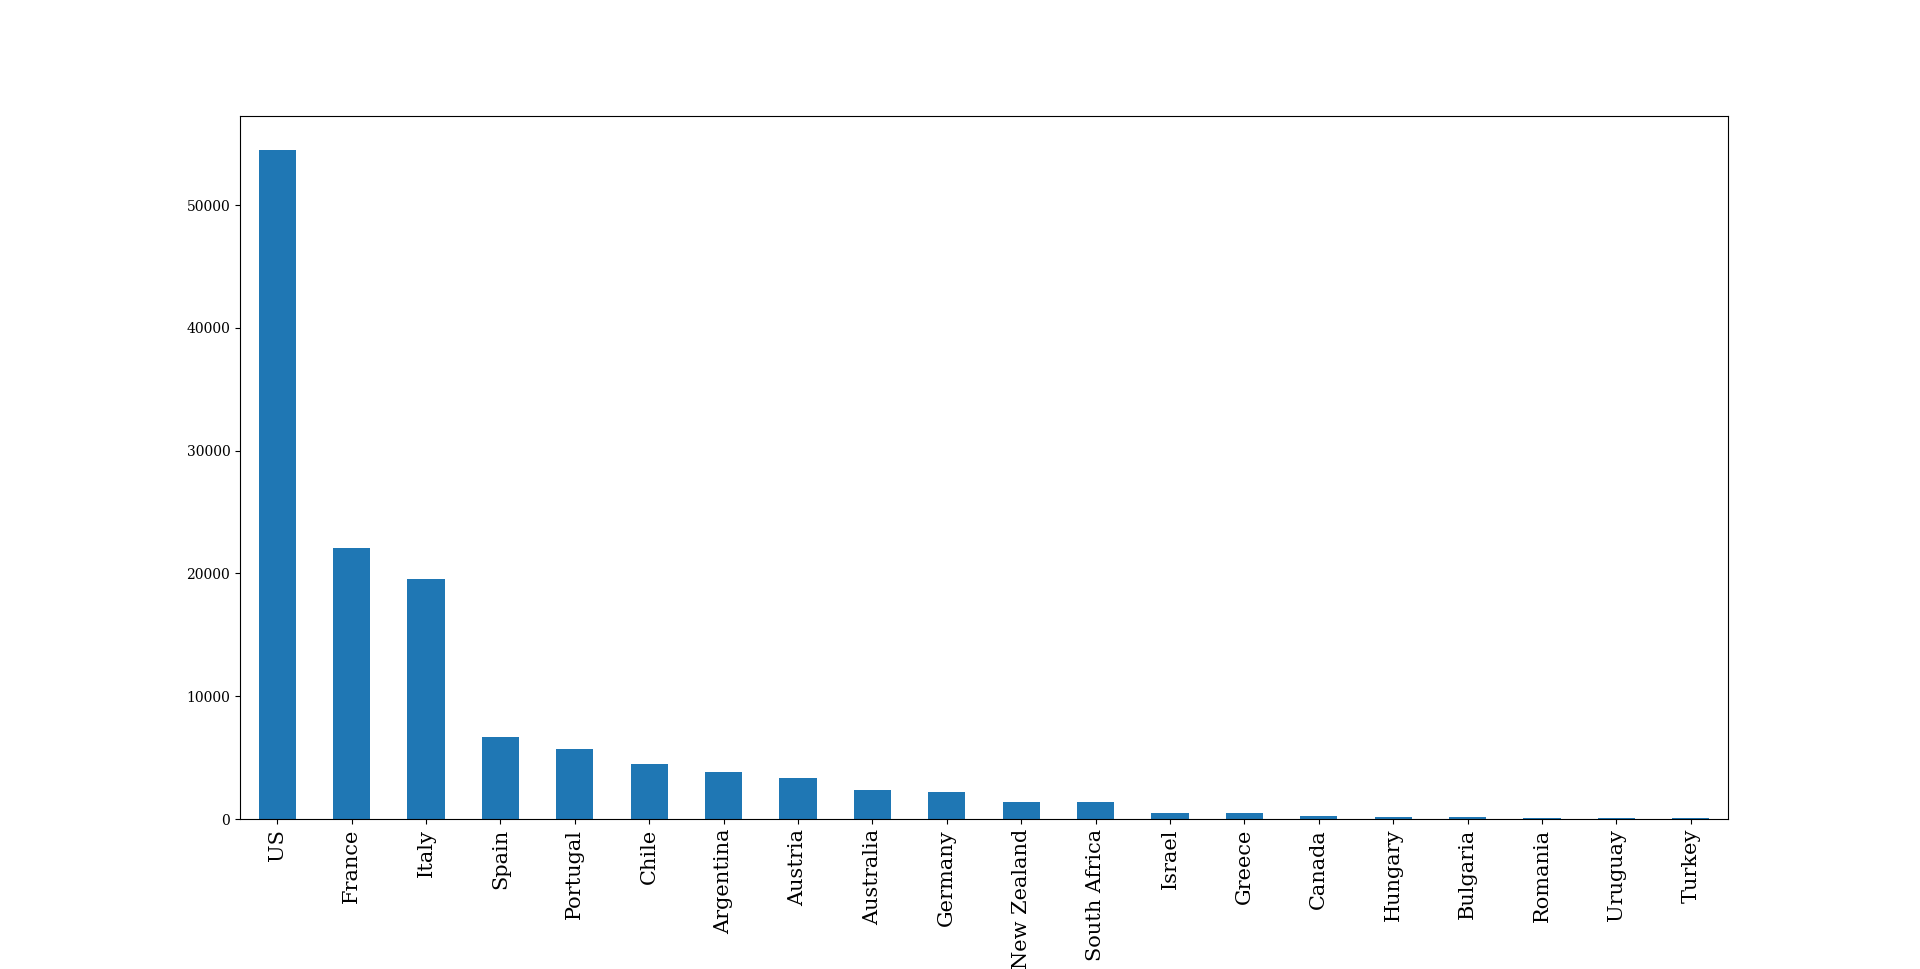
\includegraphics[width=\textwidth,height=\textheight,keepaspectratio]{figures/1c_histogram_of_country.png}

Designation

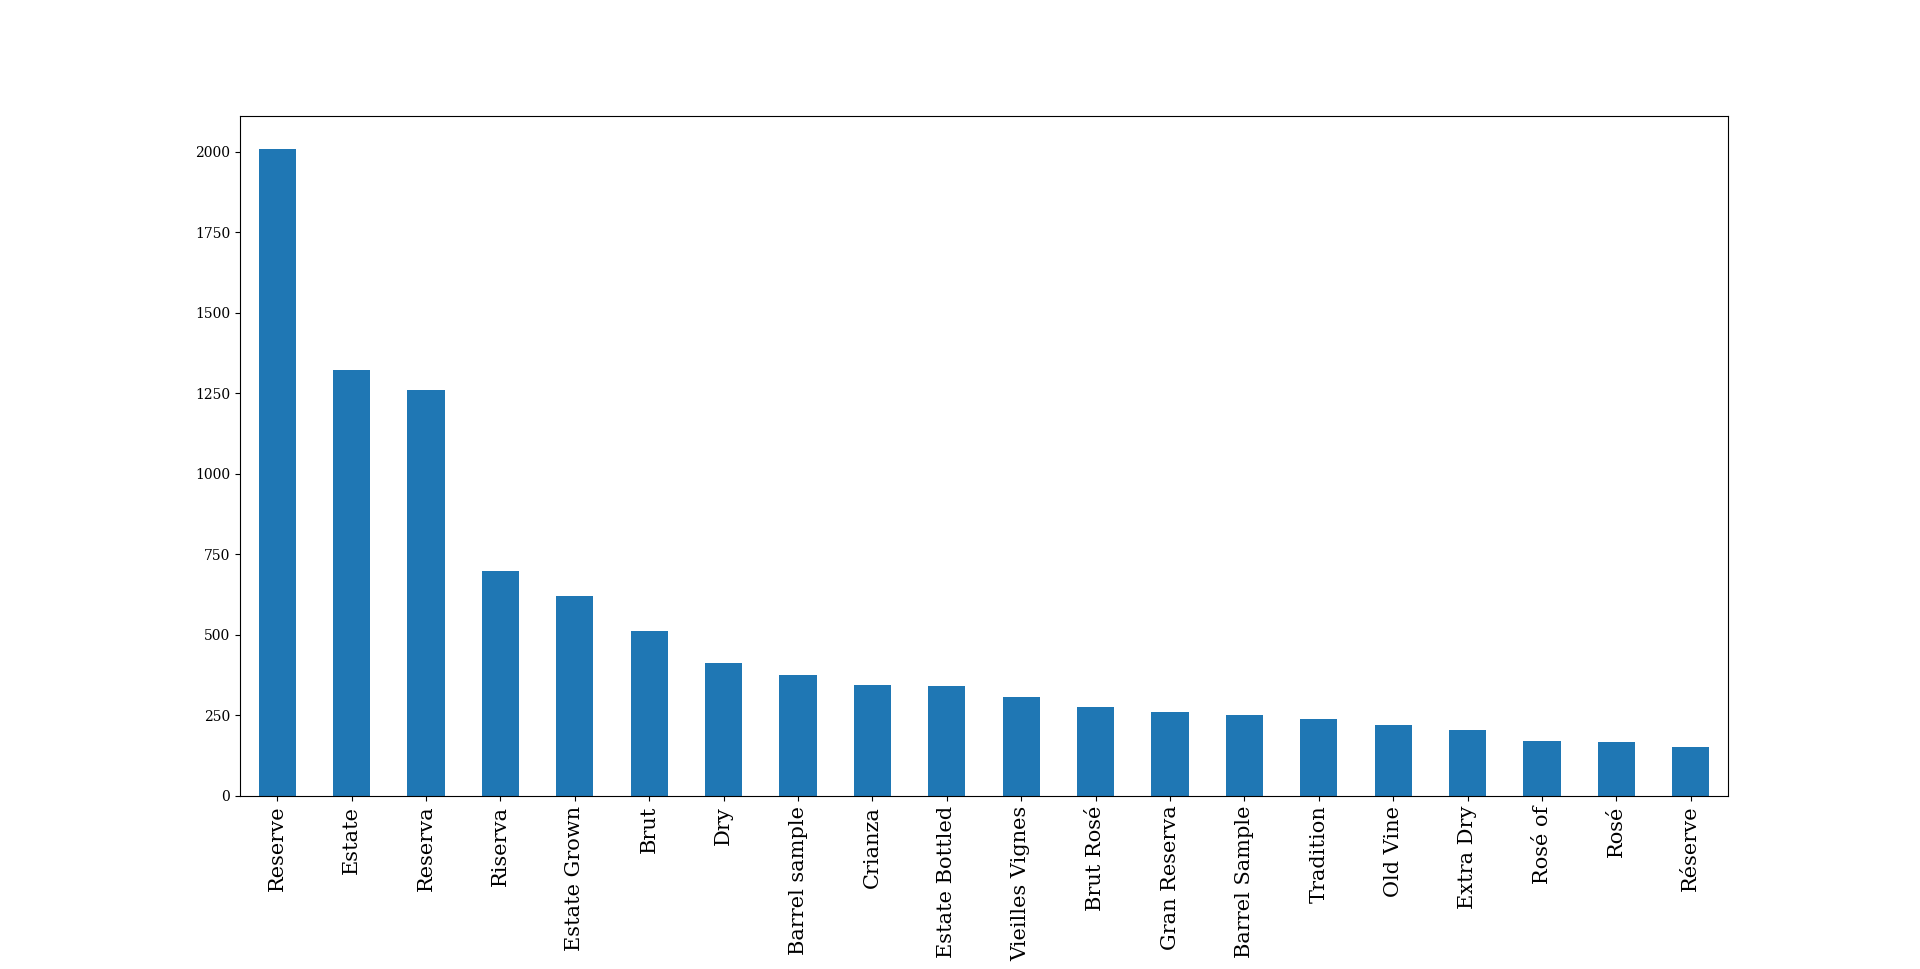
\includegraphics[width=\textwidth,height=\textheight,keepaspectratio]{figures/1c_histogram_of_designation.png}

Points

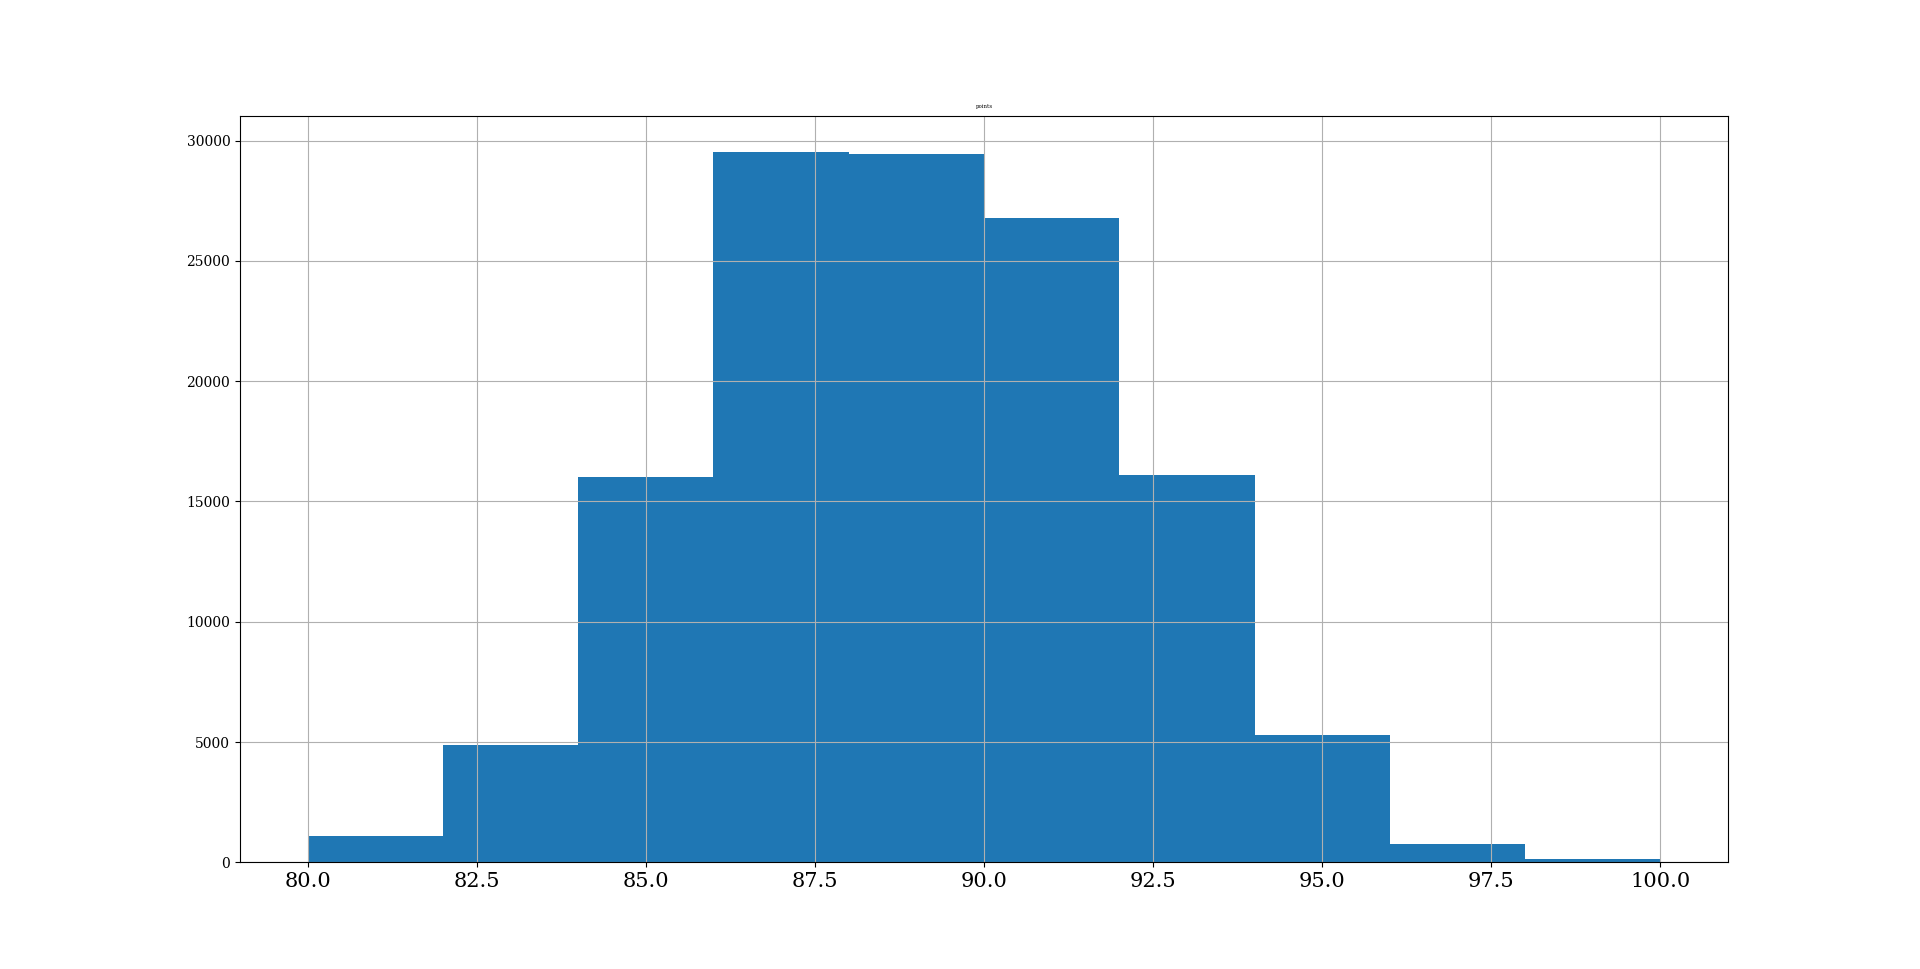
\includegraphics[width=\textwidth,height=\textheight,keepaspectratio]{figures/1c_histogram_of_points.png}

Price

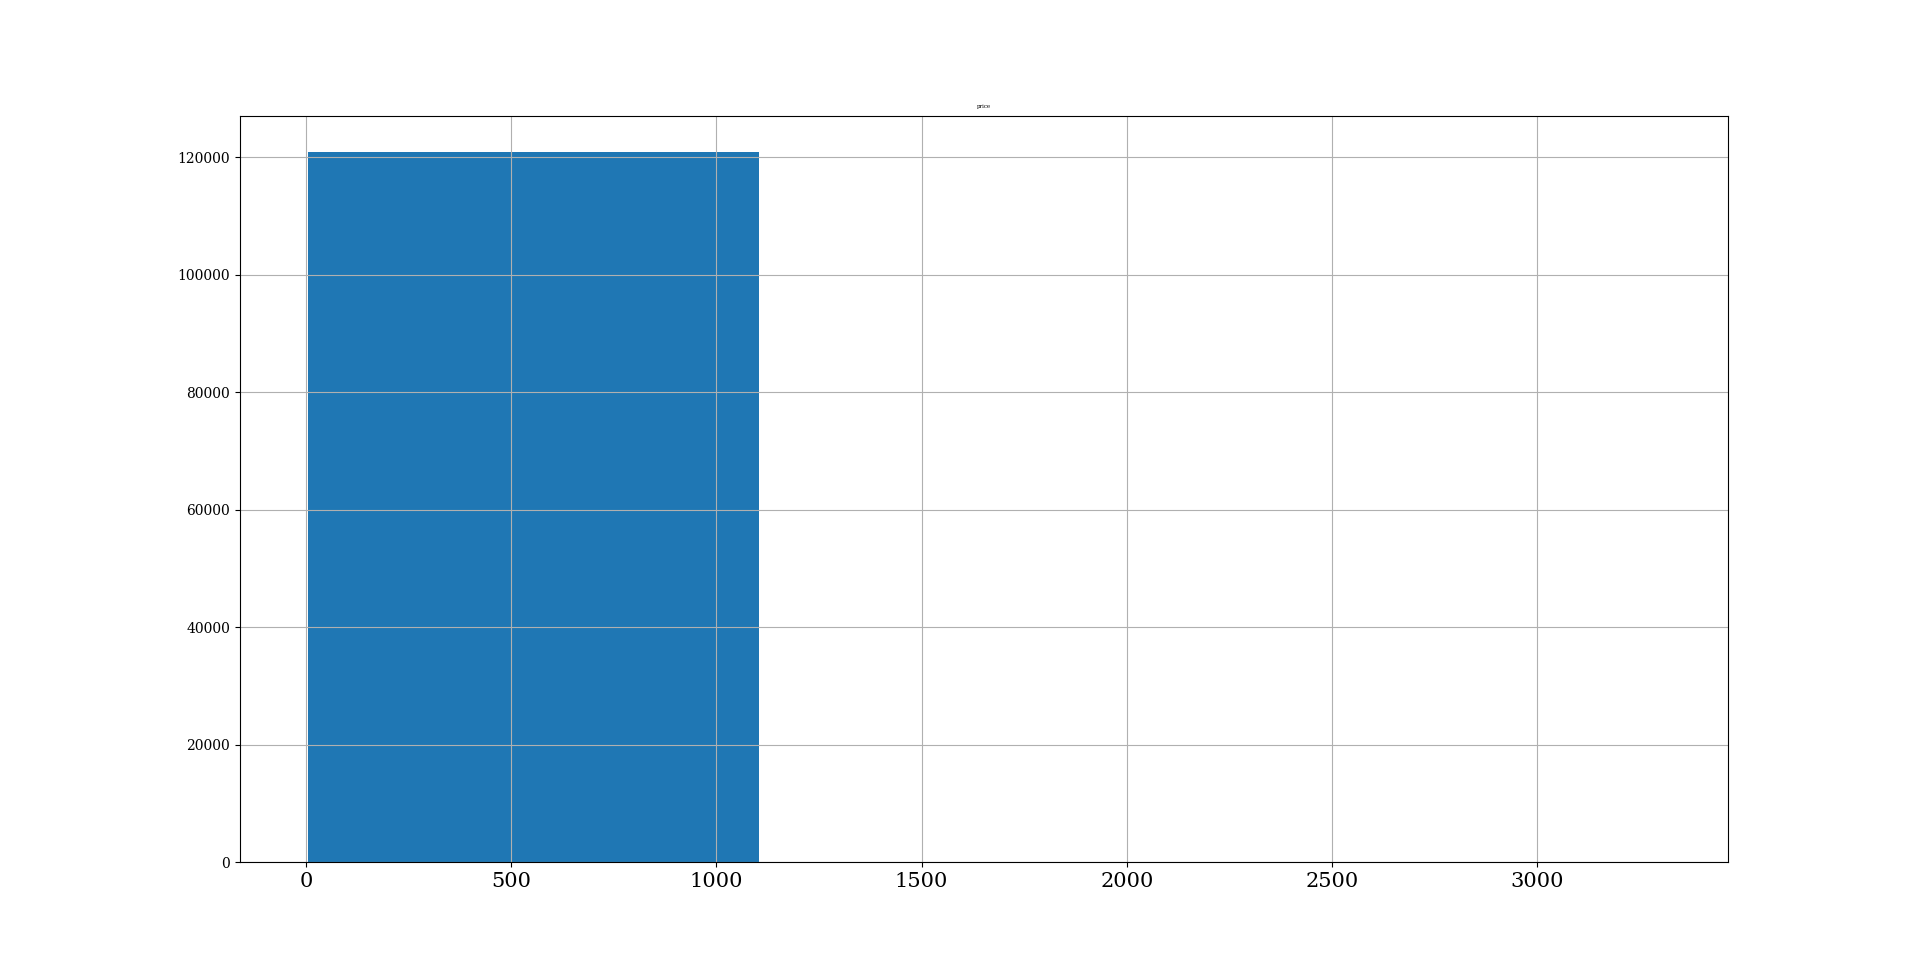
\includegraphics[width=\textwidth,height=\textheight,keepaspectratio]{figures/1c_histogram_of_price.png}

Province

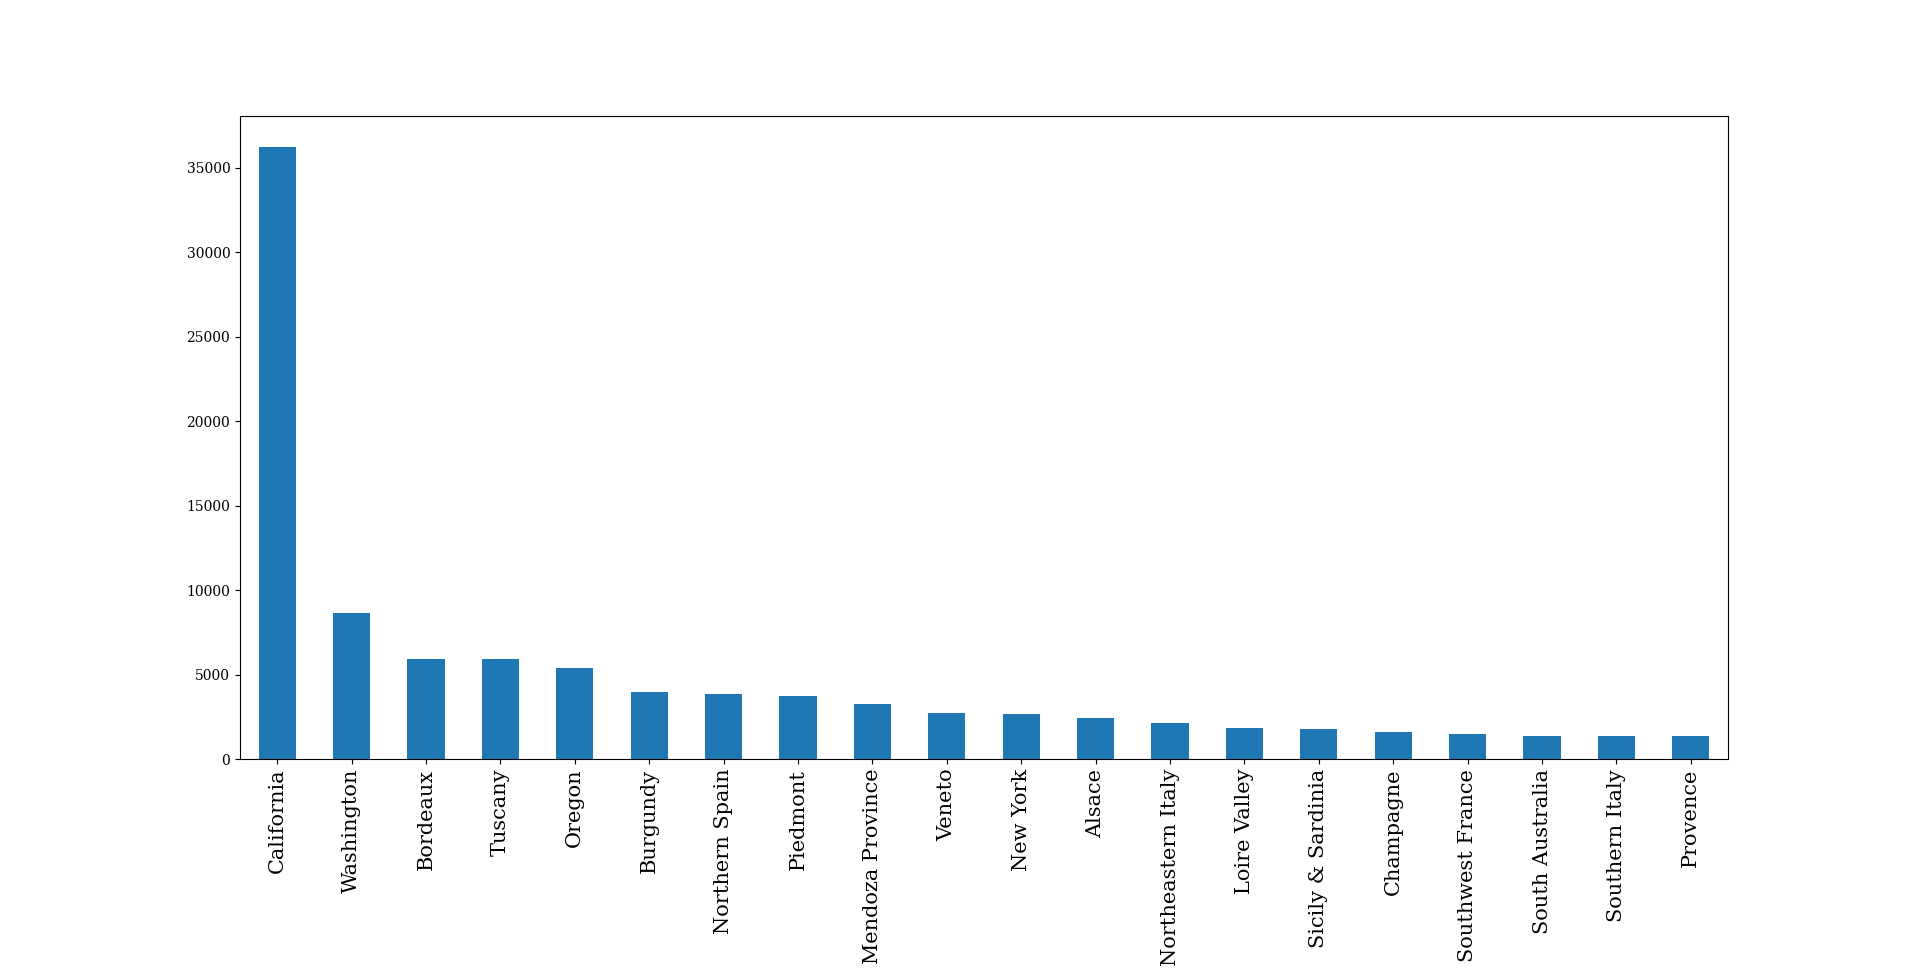
\includegraphics[width=\textwidth,height=\textheight,keepaspectratio]{figures/1c_histogram_of_province.png}

Region\_1

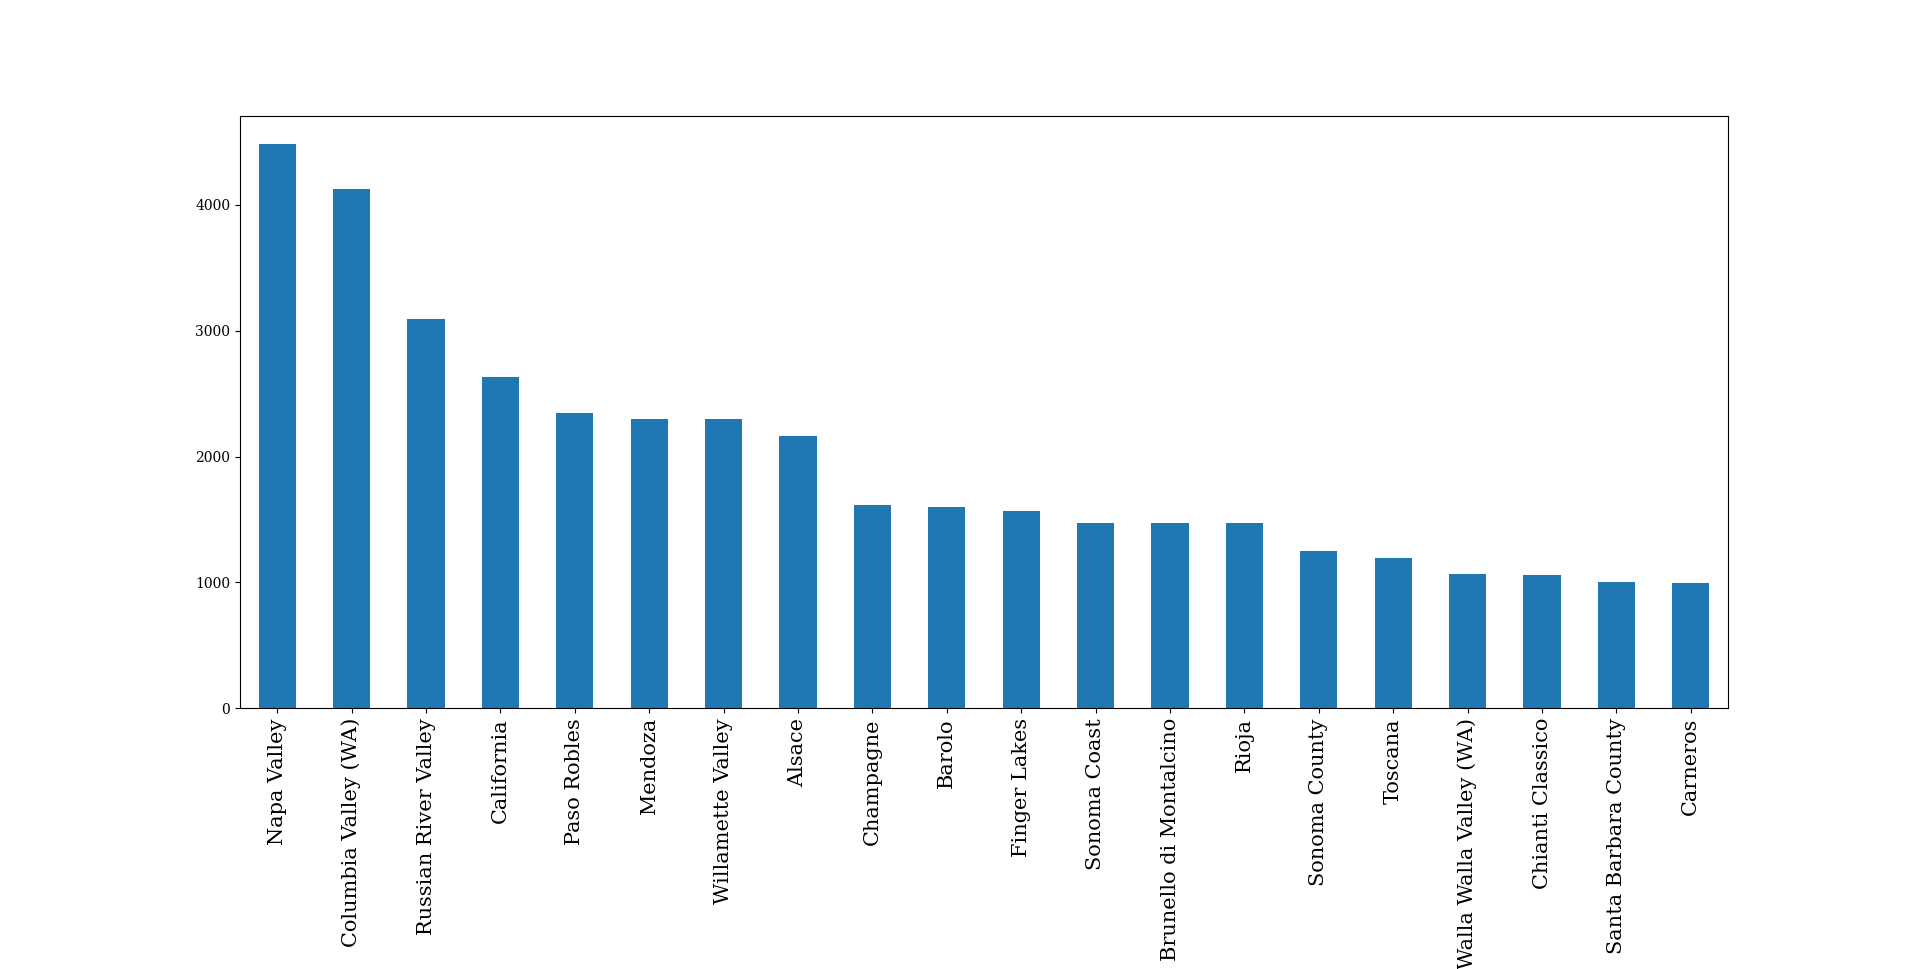
\includegraphics[width=\textwidth,height=\textheight,keepaspectratio]{figures/1c_histogram_of_region_1.png}

Region\_2

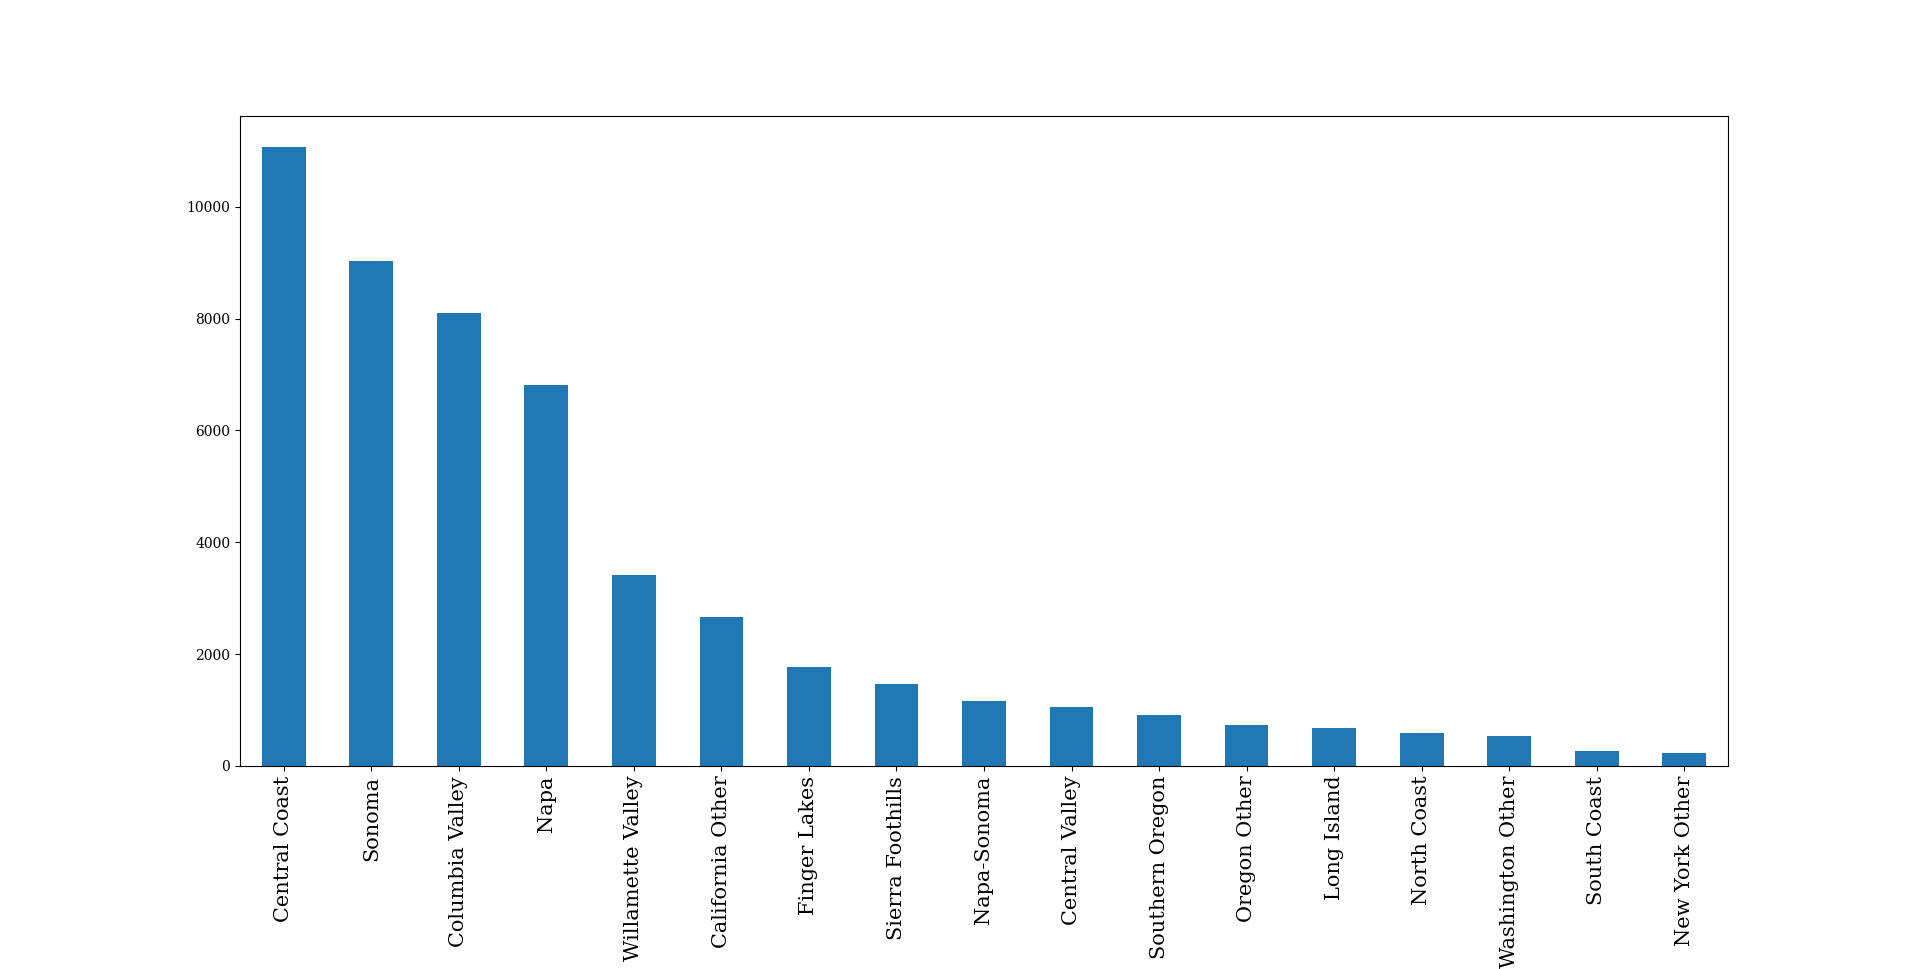
\includegraphics[width=\textwidth,height=\textheight,keepaspectratio]{figures/1c_histogram_of_region_2.png}

Taster\_name

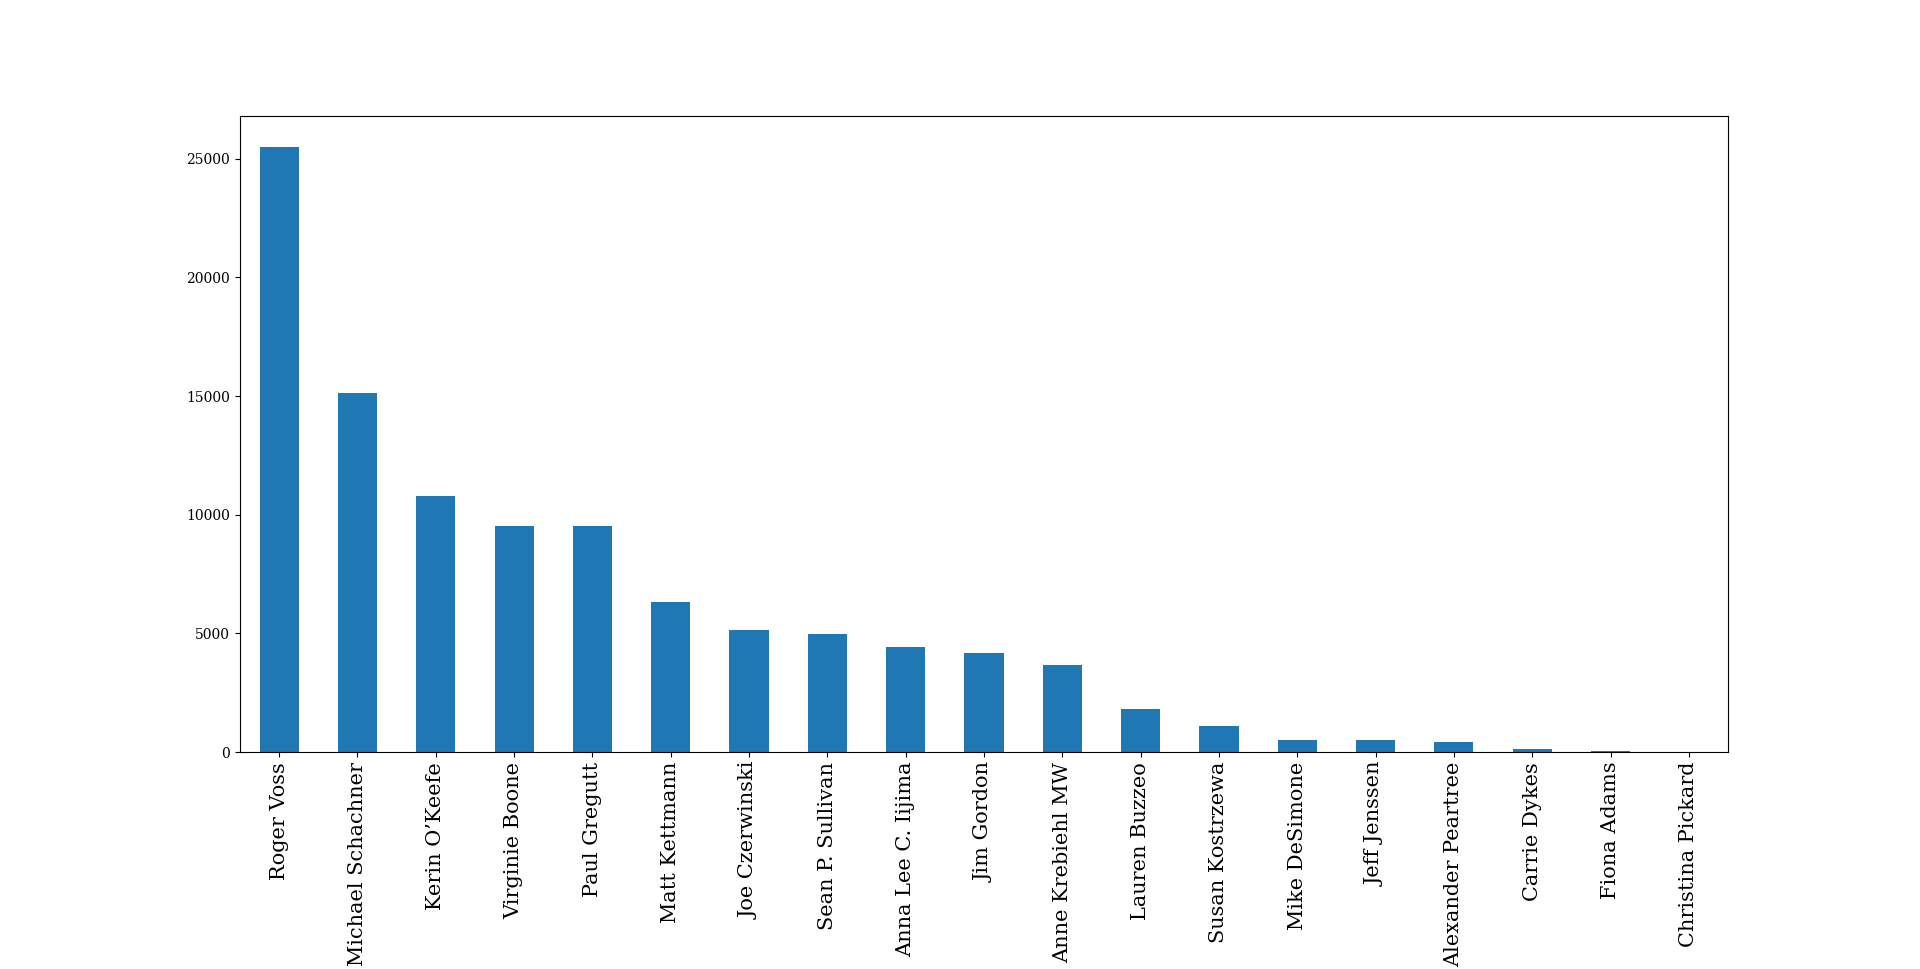
\includegraphics[width=\textwidth,height=\textheight,keepaspectratio]{figures/1c_histogram_of_taster_name.png}

Taster\_twitter\_handle

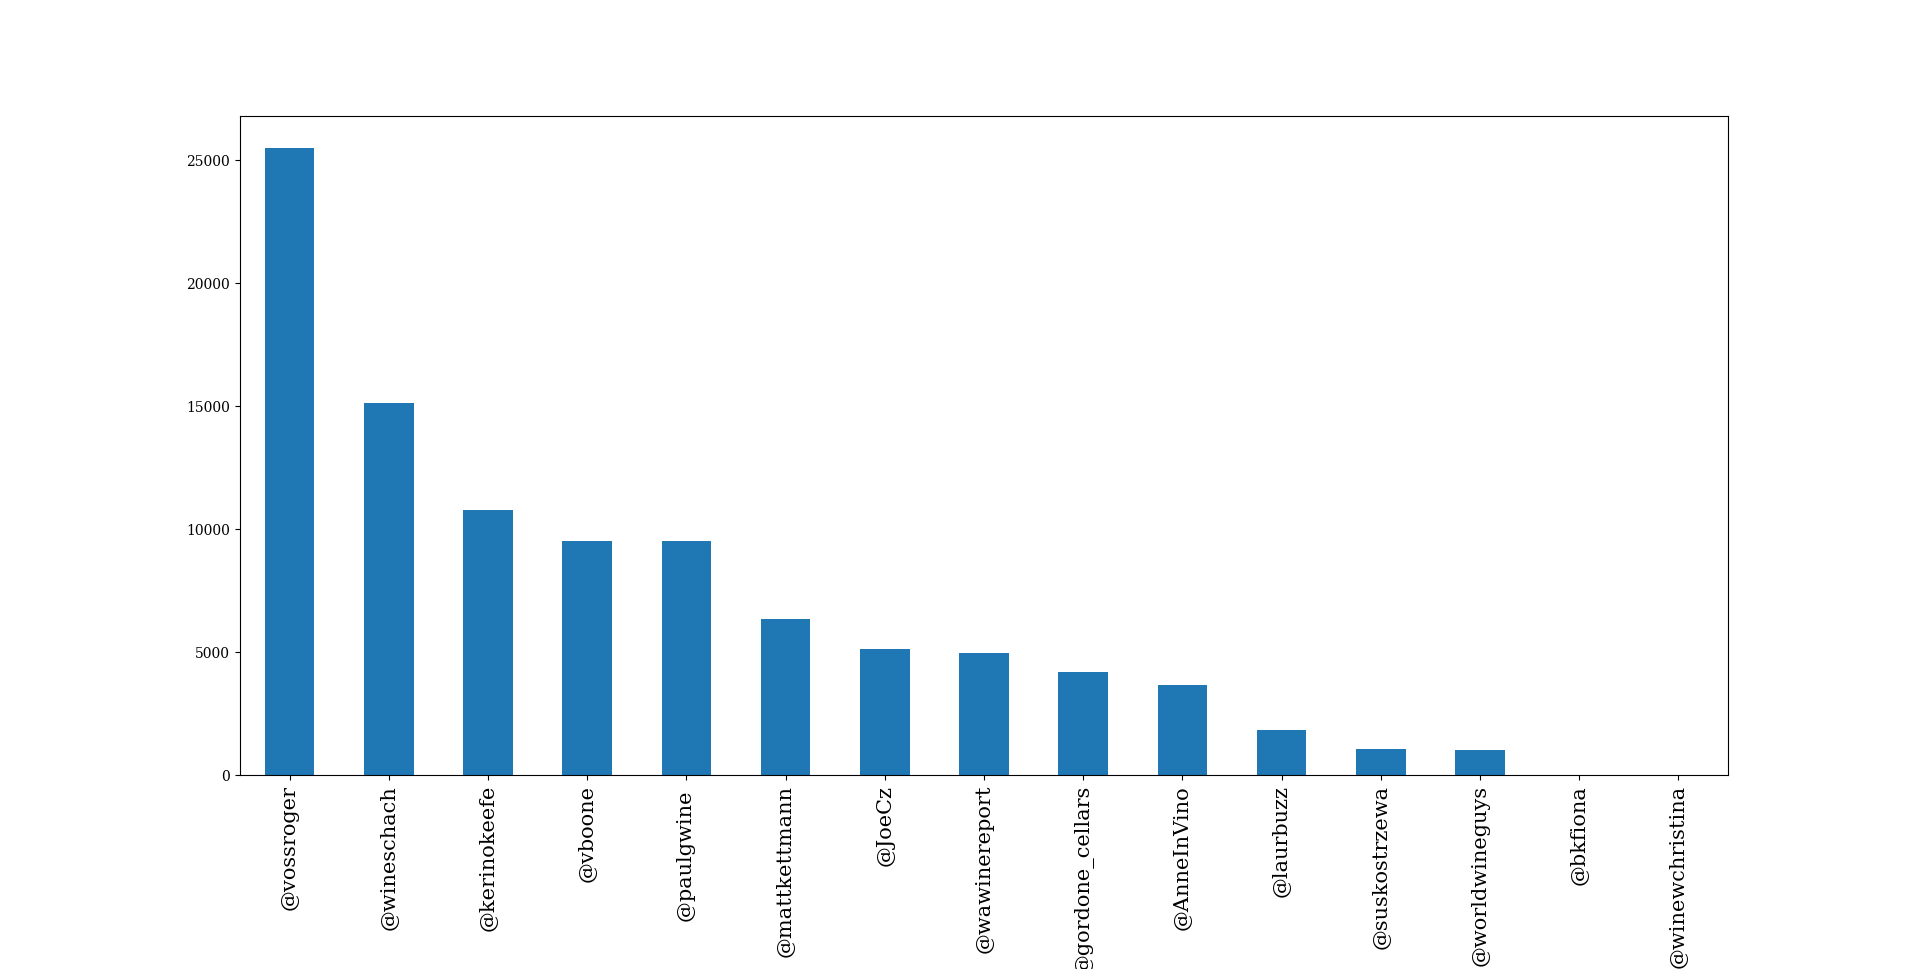
\includegraphics[width=\textwidth,height=\textheight,keepaspectratio]{figures/1c_histogram_of_taster_twitter_handle.png}

Variety

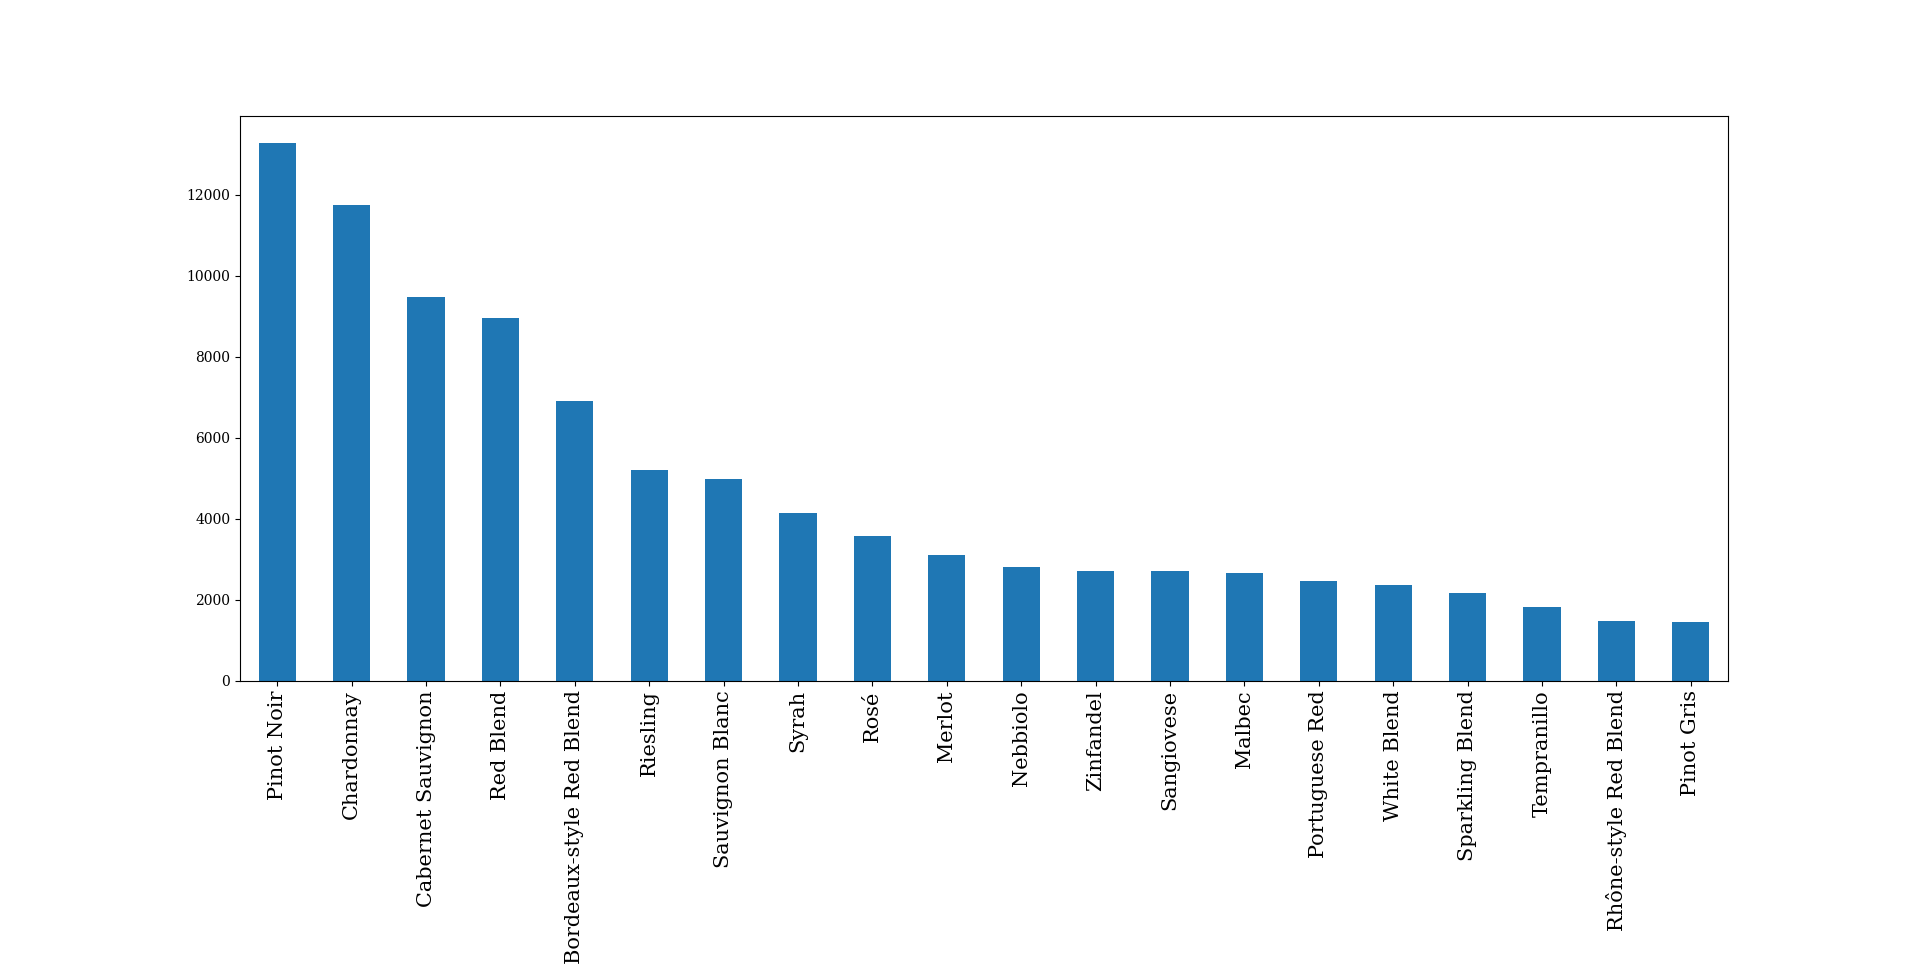
\includegraphics[width=\textwidth,height=\textheight,keepaspectratio]{figures/1c_histogram_of_variety.png}

Winery

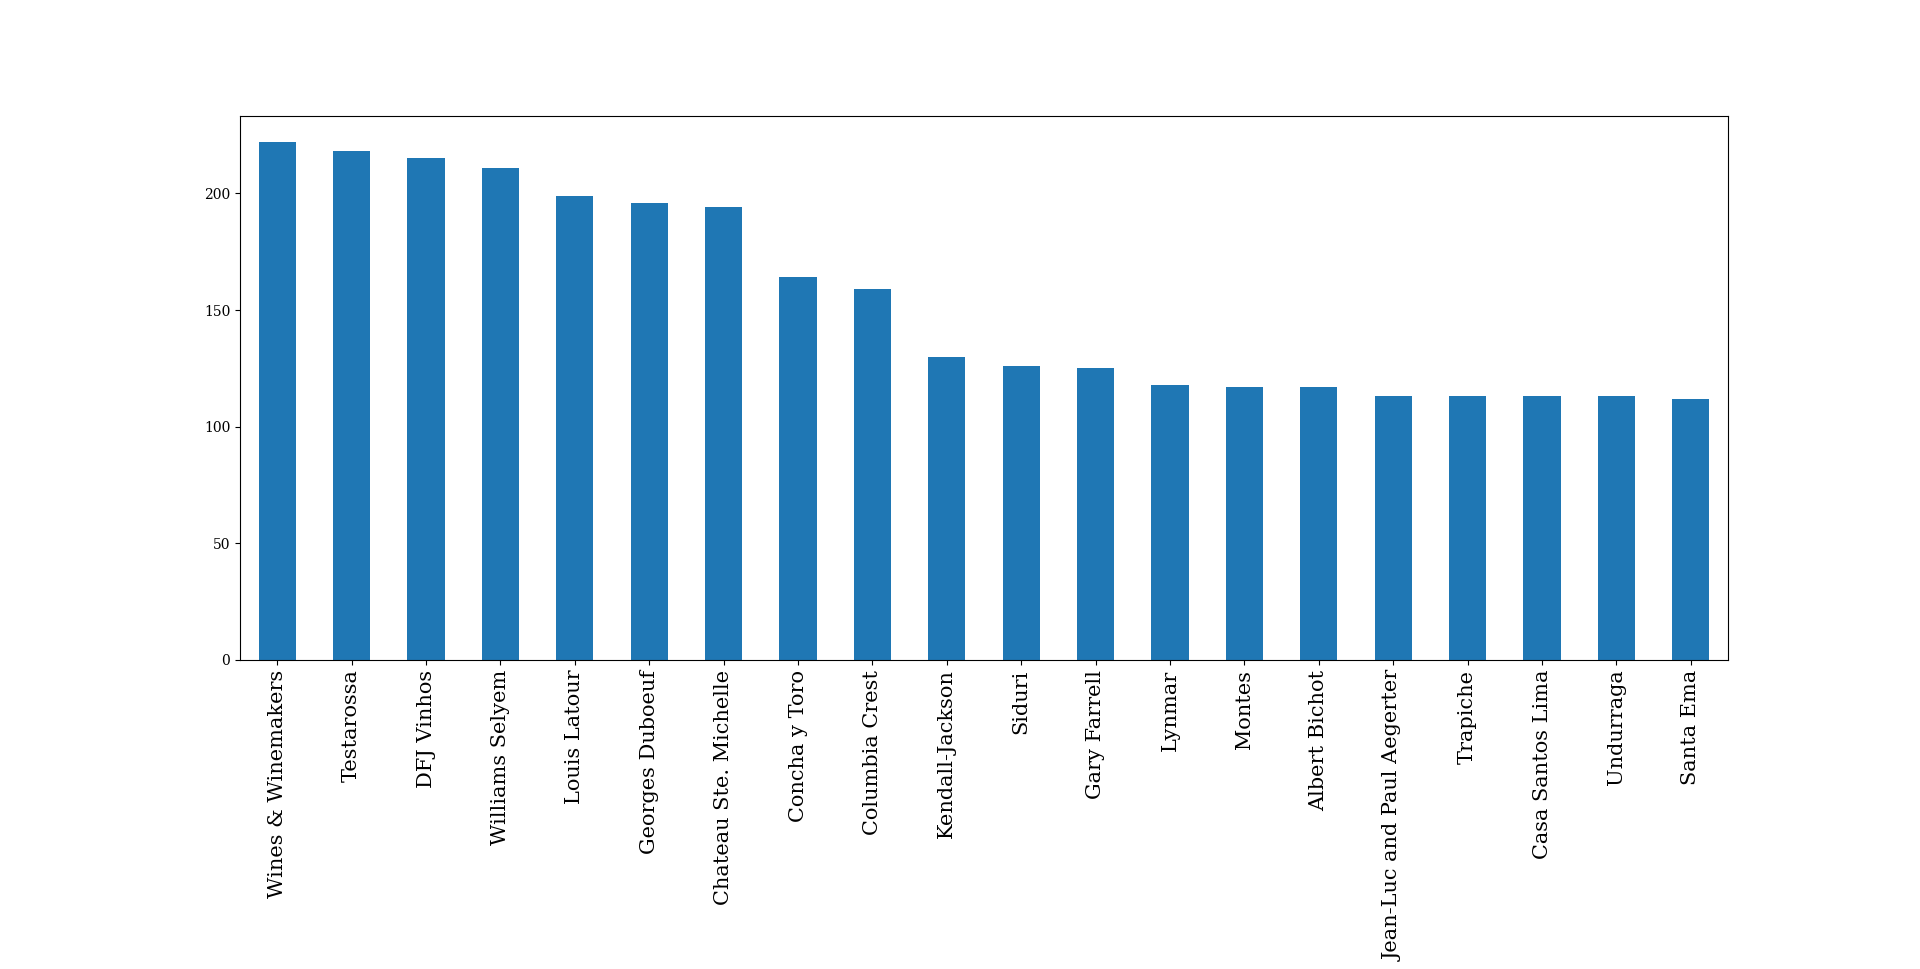
\includegraphics[width=\textwidth,height=\textheight,keepaspectratio]{figures/1c_histogram_of_winery.png}

Vintage

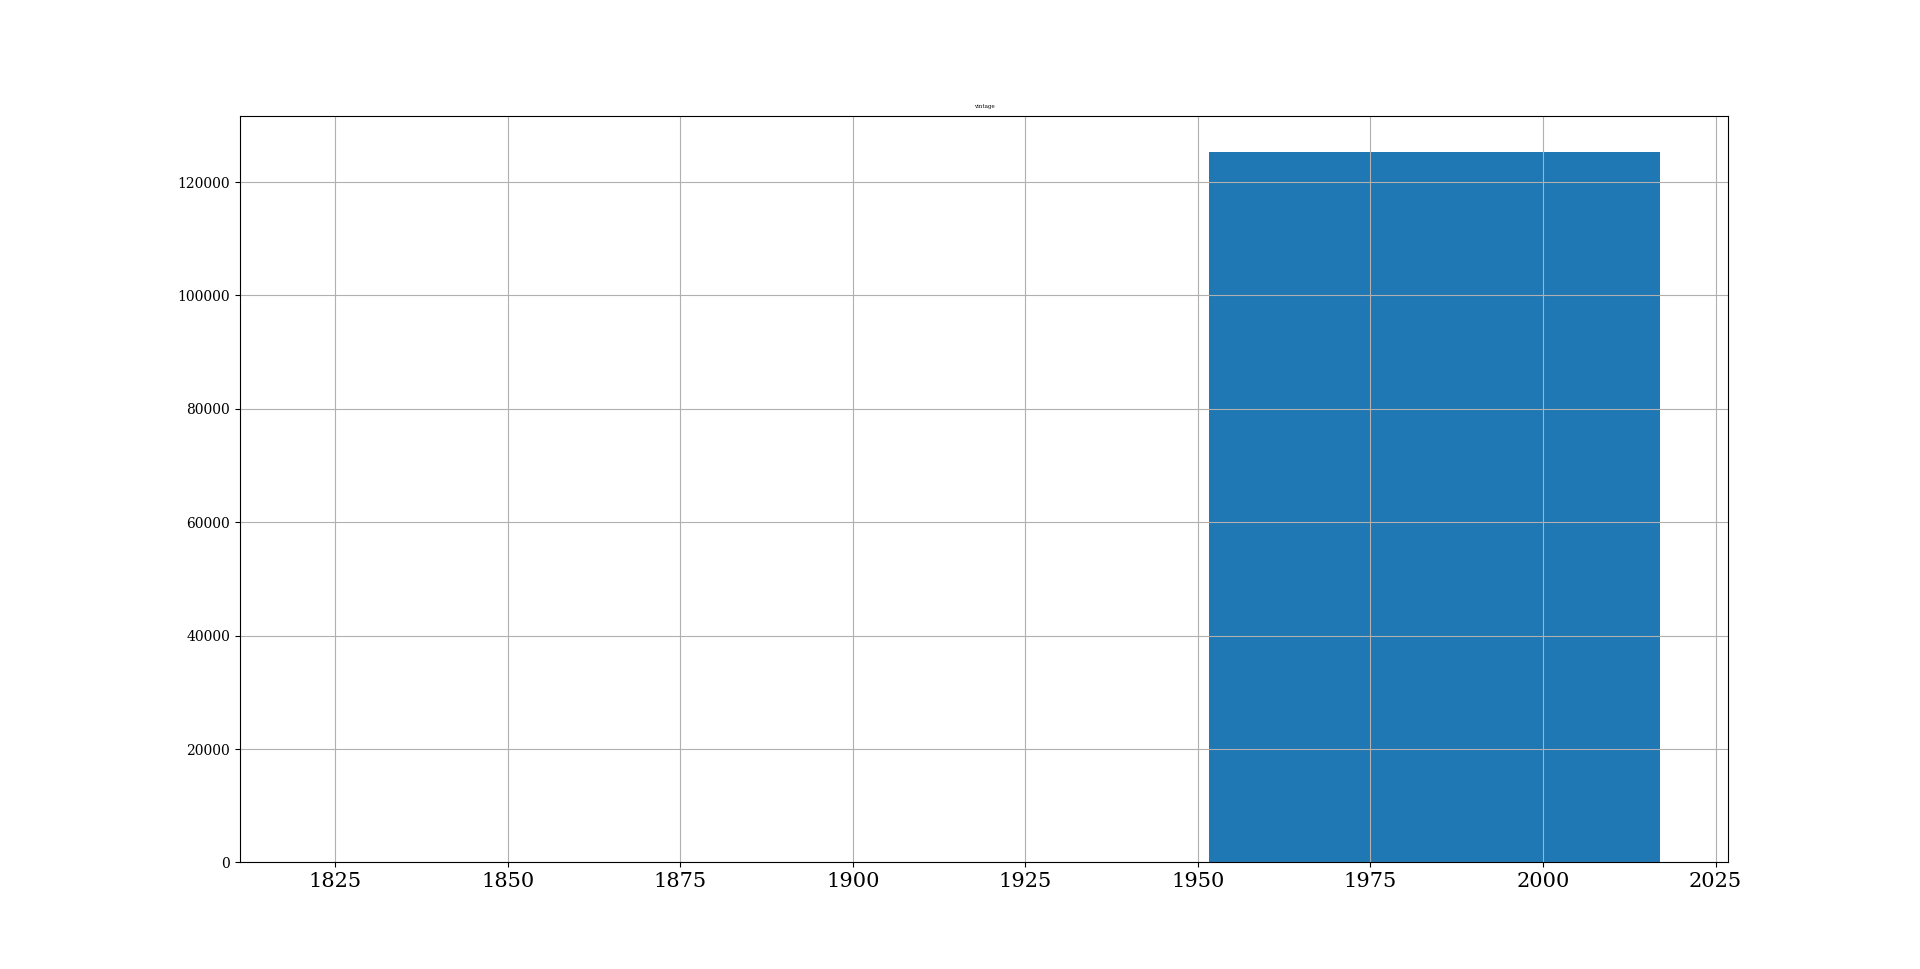
\includegraphics[width=\textwidth,height=\textheight,keepaspectratio]{figures/1c_histogram_of_vintage.png}

We also retrieve the number of null entries for each column:

\begin{itemize}
    \item country                     63
    \item description                  0
    \item designation              37465
    \item points                       0
    \item price                     8996
    \item province                    63
    \item region\_1                 21247
    \item region\_2                 79460
    \item taster\_name              26244
    \item taster\_twitter\_handle    31213
    \item title                        0
    \item variety                      1
    \item winery                       0
    \item vintage                   4611
\end{itemize}

\subsection{Statistics}
\subsection{Data Transformation}
\subsection{f}



% Print references
\end{document}
